\xchapter{Proposta}{}
\label{proposta}

Neste trabalho é proposto um módulo de identificação de momentos oportunos e inoportunos para interrupção de
motoristas, usando apenas sensores de smartphone. As seções deste capítulo estão estruturadas da seguinte forma:
A seção \ref{sec-arquitetura-solucao} apresenta a arquitetura da solução proposta. A seção \ref{sec-implementacao}
apresenta detalhes da implementação de cada módulo que compõe a solução.

\section{Momentos oportunos e inoportunos escolhidos}
\label{sec-momentos-oportunos-inoportunos}

Para a escolha dos momentos oportunos e inoportunos foi feita uma prospecção dos artigos existentes nessa área.
Nesta etapa dois artigos se mostraram promissores: O de \citeonline{kim2015sensors} e o de \citeonline{monk2004recovering}.
Ambos trabalhos citam momentos oportunos e inoportunos para detecção da interruptibilidade de motoristas.

\subsection{Momentos oportunos}
\label{subsec-momentos-oportunos}

\citeonline{kim2015sensors} desenvolveram um classificador utilizando aprendizagem de máquina para detectar a interruptibilidade
de motoristas em um dado momento. O resultado do trabalho mostrou que interrupções têm menos impacto em um motorista quando ele
não está com nenhuma das mãos no volante ou quando está interagindo com um periférico (controlador do ar condicionado, por exemplo).

Além disso, pode-se inferir a partir do trabalho de \citeonline{kim2015sensors} alguns outros momentos que são oportunos para
interromper motoristas, como por exemplo quando o carro está parado (todas as vezes em que o motorista não tinha nenhuma das
mãos no volante, a velocidade do carro era menor do que 3 km/h), quando a velocidade do veículo é baixa (durante a interação com
periféricos a velocidade do carro reduzia para cerca de 29,5 km/h) e quando a velocidade é constante.

Com base nestes achados, foi decidido que os momentos oportunos a serem detectados neste trabalho são:

\begin{itemize}
  \item Veículo parado;
  \item Veículo com velocidade menor do que 29,5 km/h e constante (sem aceleração ou desaceleração).
\end{itemize}

\subsection{Momentos inoportunos}
\label{subsec-momentos-inoportunos}

\citeonline{monk2004recovering} estudaram o efeito das interrupções e as distrações que elas causam nos motoristas. Eles concluem
em seu estudo que interrupções antes ou depois de uma tarefa ou sub-tarefa trazem menos problemas, e cita curvas, mudanças
de faixa e entrada em uma rodovia como exemplos de sub-tarefas que o motorista executa.

Com base nestas afirmações, os seguintes momentos inoportunos foram escolhidos para serem detectados no presente trabalho:

\begin{itemize}
  \item Curva;
  \item Mudança de faixa.
\end{itemize}

\section{Arquitetura}
\label{sec-arquitetura-solucao}
Segundo \citeonline{garlan1993introduction}, a arquitetura de um software é a coleção de seus componentes computacionais - ou simplesmente
componentes - junto com a descrição das interações entre estes componentes - os conectores.  Sendo assim, nesta sessão
vamos mostrar os principais elementos da solução proposta e como eles interagem entre si.

O módulo funcionará em conjunto com o aplicativo Meu Possante, um aplicativo para sistemas Android e cuja arquitetura pode ser vista
na seção \ref{meupossante-app}. A identificação dos momentos oportunos e inoportunos é feita usando apenas sensores de smartphone,
sendo que os momentos oportunos são medidos utilizando o sensor de GPS, enquanto os inoportunos usam o giroscópio.

O fluxo de dados da aplicação pode ser visto na figura \ref{arquitetura-meu-possante-com-modulo}. O fluxo começa
na coleta de dados do GPS e giroscópio, e termina na decisão de notificação ou não do usuário. As setas na
imagem representam o sentido do fluxo de dados.

\begin{figure}[h]
\centering
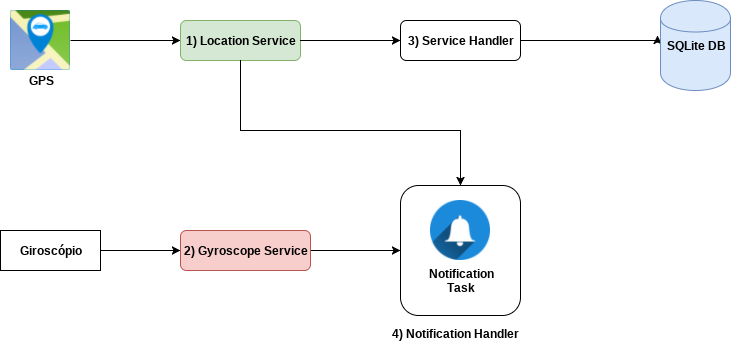
\includegraphics[width=0.8\textwidth]{images/arquitetura-meu-possante-com-modulo.png}
\caption{Arquitetura do Meu Possante após a implementação do módulo de identificação}
\label{arquitetura-meu-possante-com-modulo}
\end{figure}

Os módulos representados e suas funções são os seguintes:

\begin{enumerate}
  \item \textbf{Location Service:} Responsável pela coleta e monitoramento dos dados do GPS, incluindo deslocamento, velocidade e
  aceleração do dispositivo.
  \item \textbf{Gyroscope Service:} Responsável pela coleta e monitoramento dos dados do giroscópio. Este serviço detecta mudanças
  nos valores do sensor e aplica o algoritmo de detecção de curvas e mudanças de faixa.
  \item \textbf{Service Handler:} Responsável pela inicialização e checagem de dados dos serviços
  que estão rodando na aplicação. Este módulo também é responsável por atualizar as informações
  de quilometragem no banco de dados e chamar o módulo de notificação quando necessário.
  \item \textbf{Notification Handler:} Responsável por consultar os serviços e decidir se deve criar uma notificação ou não naquele
  momento.
\end{enumerate}

Na próxima seção são dados mais detalhes sobre a implementação dos módulos, assim como os algoritmos utilizados.

\section{Implementação}
\label{sec-implementacao}

O projeto foi desenvolvido no Android Studio, o ambiente de desenvolvimento integrado (IDE) oficial para
codificação de aplicativos Android. A linguagem utilizada foi o Java, linguagem padrão para o desenvolvimento
de aplicações Android.

As próximas subseções apresentam detalhes sobre a implementação de cada módulo que compõe a solução.

\subsection{Location Service}
\label{location-service}

O módulo \textit{Location Service} é o serviço responsável pela obtenção dos dados de GPS da aplicação. Os principais dados calculados
por este serviço são a distância percorrida desde a última leitura, o valor da velocidade e a aceleração. Esta última é necessária
apenas para determinar se a velocidade é constante ou não.

Por ser necessário obter a localização do usuário em intervalos regulares, foi preciso especificar o intervalo de tempo que o
serviço requisita atualizações da localização. Esta configuração tem impacto direto na autonomia de bateria do dispositivo,
pois quanto mais frequente é a requisição de dados do GPS, mais energia é gasta pelo dispositivo. O intervalo de tempo escolhido
foi de 5000ms (5 segundos), um intervalo razoavelmente frequente e que preserva a autonomia de bateria.

A distância percorrida é um dado necessário para o Meu Possante calcular a quilometragem percorrida pelo veículo até o momento e
sinalizar as trocas de peças quando necessário. Já os valores de velocidade e aceleração são necessários para determinar se um
momento é oportuno ou inoportuno para notificar um motorista. A relação entre os momentos e os dados que são usados para
identificá-los estão relacionados na tabela \ref{tabela-momentos-dados}.

\begin{table}[h]
\centering
\caption{Relação entre momentos oportunos e dados necessários para identificá-los}
\label{tabela-momentos-dados}
\begin{tabular}{|c|c|}
\hline
\textbf{Momento oportuno}                     & \textbf{Dado do serviço utilizado} \\ \hline
Veículo parado                                & Velocidade                         \\ \hline
Velocidade constante e menor do que 29,5 km/h & Velocidade e aceleração            \\ \hline
\end{tabular}
\end{table}

Mais informações sobre os referidos momentos podem ser lidas na seção \ref{sec-momentos-oportunos-inoportunos}.

Dois métodos importantes deste módulo são o \lstinline[basicstyle=\ttfamily\color{black}]|isAccelerating()|, que retorna um valor
booleano que julga se o veículo está acelerando ou não, e o método \lstinline[basicstyle=\ttfamily\color{black}]|getLastSpeed()|, que
retorna a última velocidade medida do veículo. Estes dois métodos são utilizados pelo módulo \textit{Notification Handler} para decidir se
a notificação pode ser disparada ou não.

Os valores de velocidade e distância percorrida são dados por métodos padrões da API Location, a API padrão para se trabalhar
com dados de geo-referenciamento em Android. Entretanto, não há um método padrão nesta API para medir a aceleração, e por este
motivo foi necessária a criação de um método para calculá-la. O método foi estruturado da seguinte forma:

\begin{enumerate}
  \item As últimas 5 leituras de velocidade são sempre guardadas;
  \item Verifica-se a variação de velocidade entre elas;
  \item Caso a variação entre uma leitura e sua subsequente seja menor do que 5 km/h mais o desvio padrão das leituras em questão,
  considera-se que a velocidade é constante naquele momento.
\end{enumerate}

Caso a aceleração seja constante e a velocidade seja menor que 29,5 km/h, significa que o momento é oportuno para notificar o motorista

\subsection{Gyroscope Service}
\label{gyroscope-service}

Este serviço é o responsável pela obtenção dos dados de giroscópio. Este é o módulo mais complexo desta proposta, por ser o responsável por
detectar se o veículo está fazendo uma curva ou mudança de faixa usando apenas os dados do giroscópio. O algoritmo usado para identificar
estes dois momentos inoportunos foi desenvolvido por \citeonline{chen2015invisible} e adaptado para este trabalho.

\citeonline{chen2015invisible} relatam em seu trabalho que quando um carro muda de direção (ex: ao mudar de faixa, fazer uma curva ou passar
por rodovias sinuosas), o eixo Z do giroscópio pode ser usado para representar a velocidade angular do veículo para aquela mudança de direção.
Eles também perceberam que o padrão das leituras deste eixo se repete para determinadas atividades, como curvas e mudanças de faixa, como pode
ser visto na figura \ref{leituras-giroscopio}.

\begin{figure}[h]
\centering
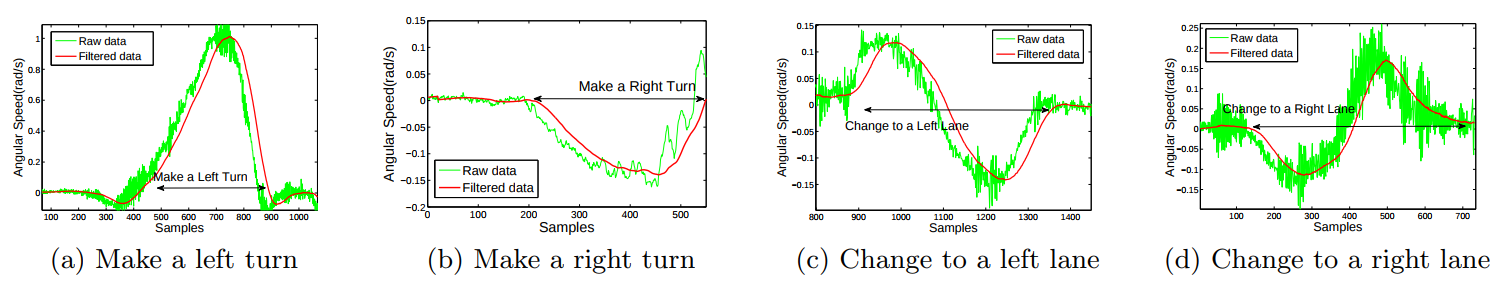
\includegraphics[width=1\textwidth]{images/leituras-giroscopio.png}
\caption{Leituras do giroscópio quando o veículo faz uma curva à direita/esquerda ou mudança de faixa à direita/esquerda \cite{chen2015invisible}}
\label{leituras-giroscopio}
\end{figure}

Pode-se observar na figura \ref{leituras-giroscopio} que as curvas são caracterizadas por uma alteração nas leituras, sendo esta positiva ou negativa,
a depender do sentido da curva; enquanto que a mudança de faixa caracteriza-se por duas alterações sequenciais, sendo a segunda no sentido inverso
da primeira.

Observando estes padrões, \citeonline{chen2015invisible} desenvolveram um conjunto de regras que determina se a alteração nas leituras do eixo Z do
giroscópio pode ser considerada um indicador de curva ou mudança de faixa. As regras são as seguintes:

\begin{enumerate}
  \item Todas as leituras durante a alteração devem ser maiores que $\delta_{s}$;
  \item O maior valor registrado durante a alteração deve ser maior do que $\delta_{h}$;
  \item A duração de uma alteração não deve ser menor do que $T_{BUMP}$.
\end{enumerate}

Através de testes e experimentos, os valores ideais encontrados por \citeonline{chen2015invisible} para as variáveis acima foram de $\delta_{s}$ = 0.05 rad/s,
$\delta_{h}$ = 0.07 rad/s e $T_{BUMP}$ = 1.5 segundos.

Considerando estas regras para o que é considerada uma alteração válida, \citeonline{chen2015invisible} desenvolveram um algoritmo baseado em mudança de estados
que tenta identificar quando o veículo está fazendo uma curva ou mudança de faixa. O algoritmo está representado na figura \ref{algoritmo-giroscopio}.

\begin{figure}[h]
  \centering
  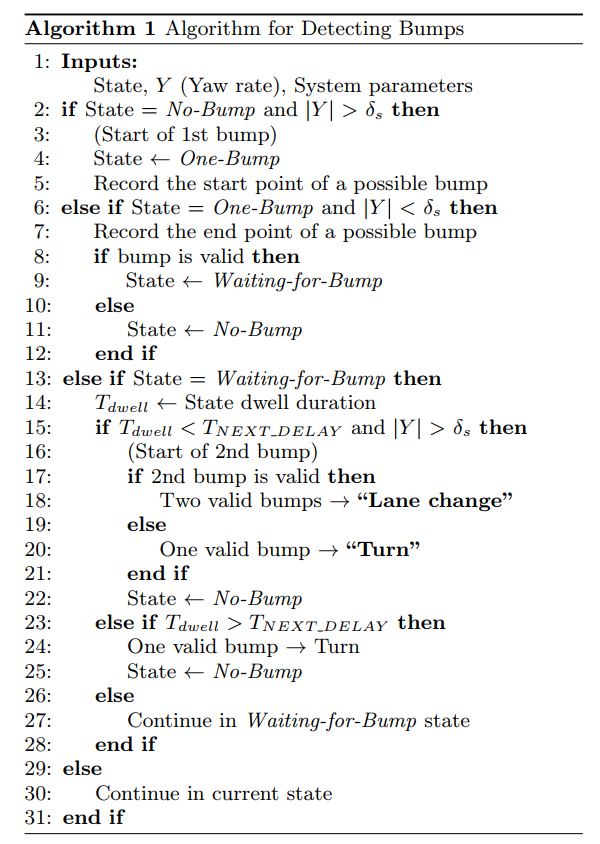
\includegraphics[width=0.45\textwidth]{images/algoritmo-giroscopio.png}
  \caption{Algoritmo de detecção de curvas e mudanças de faixa \cite{chen2015invisible}}
  \label{algoritmo-giroscopio}
\end{figure}

Os três estados do algoritmo são os seguintes:

\begin{itemize}
  \item \textbf{No-Bump:} Neste estado, nenhuma alteração foi detectada até o momento. Caso o valor do giroscópio passe de $\delta_{s}$, a alteração começa a ser
  monitorada e o estado passa a ser \textit{One Bump};
  \item \textbf{One-Bump:} Este estado começa quando o valor do giroscópio passa de $\delta_{s}$ e termina quando o valor volta a ser menor do que $\delta_{s}$.
  Caso as três regras definidas para uma alteração ser válida forem satisfeitas, o estado passa a ser \textit{Waiting-for-Bump}, caso contrário o estado volta
  a ser \textit{No-Bump}.
  \item \textbf{Waiting-for-Bump:} Este estado sucede o de \textit{One-Bump} e monitora as leituras do valor do giroscópio por um tempo de 3 segundos. Caso
  uma outra alteração comece durante esse intervalo de tempo, a alteração começa a ser monitorada. Caso ela seja válida, significa que duas alterações válidas
  ocorreram seguidamente, o que caracteriza uma mudança de faixa. Caso contrário, significa que apenas uma alteração válida ocorreu, o que caracteriza uma curva.
\end{itemize}

A solução proposta pelo presente trabalho utiliza o algoritmo de \citeonline{chen2015invisible} para detectar os momentos inoportunos de notificação: curva
e mudança de faixa. O método \lstinline[basicstyle=\ttfamily\color{black}]|isAbleToNotify()| é o responsável por informar ao módulo \textit{Notification Handler}
se o momento atual é oportuno ou não.

\subsection{Service Handler}
\label{service-handler}

\subsection{Notification Handler}
\label{notification-handler}
